\documentclass[tikz,convert={density=150,size=600,outext=.png}]{standalone}
\usetikzlibrary{shapes, calc, arrows, fit, positioning, decorations, patterns, decorations.pathreplacing, chains, snakes}

\begin{document}
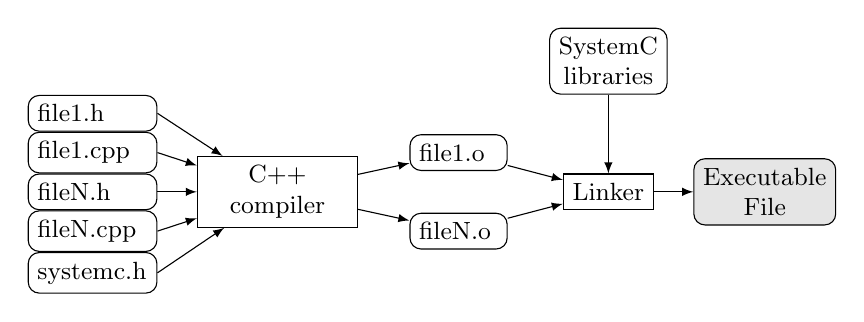
\begin{tikzpicture}[scale=1.0, >=latex, font=\small]

\begin{scope}[text width=1.4cm]
    \node[draw, rounded corners] (file1-h) {file1.h};
    \node[draw, rounded corners, below= 0cm of file1-h.south west, anchor=north west] (file1-cpp) {file1.cpp};
    \node[draw, rounded corners, below= 0cm of file1-cpp.south west, anchor=north west] (fileN-h) {fileN.h};
    \node[draw, rounded corners, below= 0cm of fileN-h.south west, anchor=north west] (fileN-cpp) {fileN.cpp};
    \node[draw, rounded corners, below= 0cm of fileN-cpp.south west, anchor=north west] (systemc-h) {systemc.h};
\end{scope}
    
\node[draw, right = 0.5cm of fileN-h, text width=1.8cm, align=center] (compiler) {C++ \\ compiler};

\begin{scope}[text width=1.cm]
    \node[draw, rounded corners, right= 3.2cm of file1-cpp] (file1-o) {file1.o};
    \node[draw, rounded corners, right= 3.2cm of fileN-cpp] (fileN-o) {fileN.o};
\end{scope}

\node[draw, right = 2.6cm of compiler,] (linker) {Linker};
\node[draw, rounded corners, above = of linker, align=center] (libs) {SystemC \\ libraries};

\node[draw, rounded corners, right = 0.5cm of linker, align=center, fill=black!10] (exe) {Executable\\File};

\draw[->] (file1-h.east) -- (compiler);
\draw[->] (file1-cpp.east) -- (compiler);
\draw[->] (fileN-h.east) -- (compiler);
\draw[->] (fileN-cpp.east) -- (compiler);
\draw[->] (systemc-h.east) -- (compiler);
    
\draw[->] (compiler) -- (file1-o);
\draw[->] (compiler) -- (fileN-o);

\draw[->] (file1-o) -- (linker);
\draw[->] (fileN-o) -- (linker);

\draw[->] (libs) -- (linker);
\draw[->] (linker) -- (exe);

\end{tikzpicture}

\end{document}
